empieza el 4

\subsection{Ecualizador de Fase}


\begin{figure}[H]
	\centering
	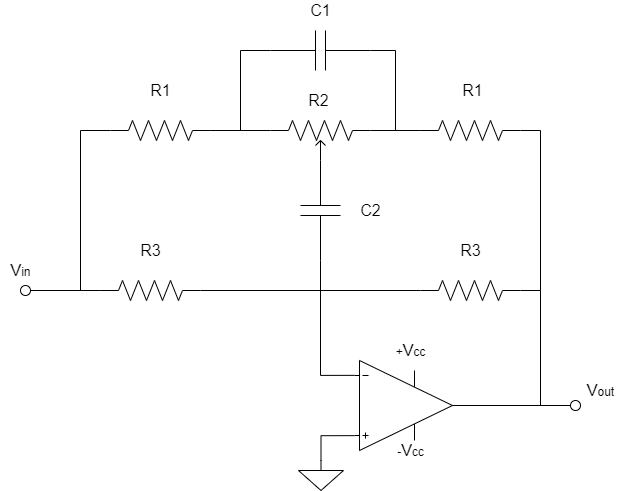
\includegraphics[scale=1]{../Ejercicio4-EcualizadorDeFase/Informe/Ecualizador de Fase.png}
	\caption{Circuito Ecualizador de Fase}
\end{figure}


\subsection{Análisis matemático}

Para analizar el circuito propuesto, se opto por reemplazar la resistencia variable $R_2$ por dos resistencias las cuales llamaremos $R_{21}$ y $R_{22}$, de esta forma será más fácil poder resolver el circuito propuesto, para esto definimos:

\begin{align}

	\begin{equation}
		R_{21} = R_2 . \delta
	\end{equation}

	\begin{equation}
		R_{22}= R_2 . (1 - \delta)
	\end{equation}

\end{align}


\begin{figure}[H]
	\centering
	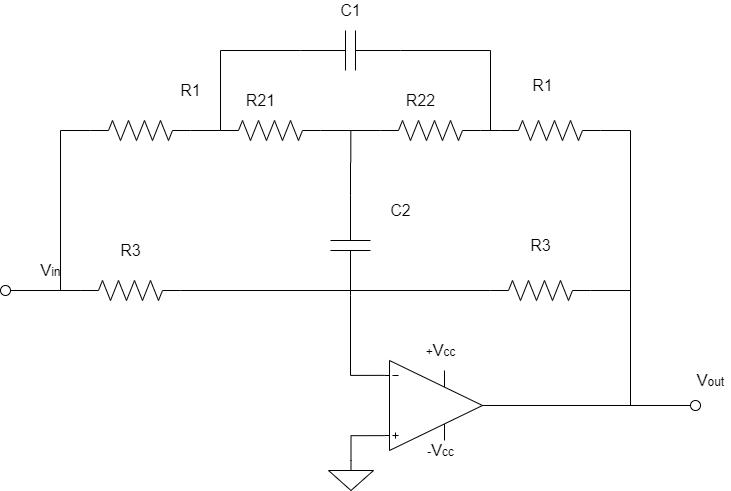
\includegraphics[scale=1]{../Ejercicio4-EcualizadorDeFase/Informe/EcSinPot.png}
	\caption{Modelo matemático}
\end{figure}

Se utilizo el reemplazo de impedancia de configuración triangulo a estrella y luego una transformación de configuración estrella a triangulo como se muestra en las imágenes \ref{1reemplazo} y \ref{2reemplazo}  para poder simplificar el circuito lo mas posible el circuito.
Para el primer reemplazo se usaron las siguientes ecuaciones:

\begin{align}

	\begin{equation}
		Z_{AB}= \frac{1}{sC_1}
	\end{equation}

	\begin{equation}
		Z_{BC}= R_{22}
	\end{equation}
	
	\begin{equation}
		Z_{CA}= R_{21}
	\end{equation}

\end{align}

\begin{figure}[h]
	\caption{1° Reemplazo}
	\centering
	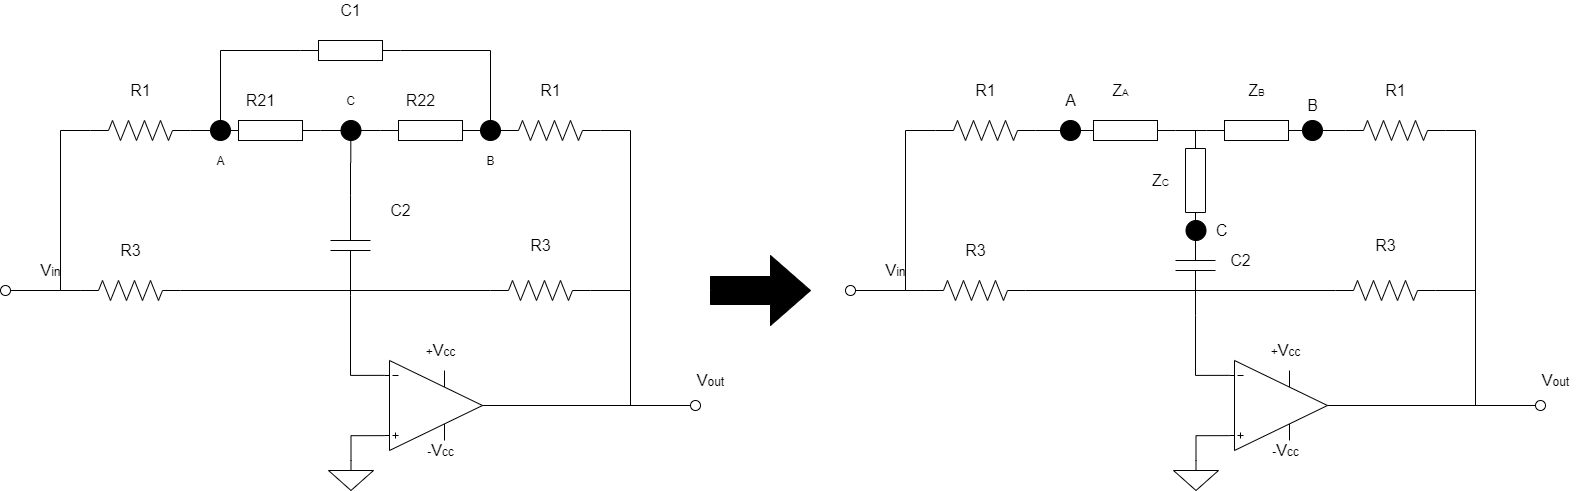
\includegraphics[scale=0.6]{../Ejercicio4-EcualizadorDeFase/Informe/1cambioEstrella.png}
	\label{1reemplazo} 
\end{figure}

Para el segundo reemplazose usaron las siguientes ecuaciones:

\begin{align}

	\begin{equation}
		Z_{A'}= R_1 + Z_{A}
	\end{equation}

	\begin{equation}
		Z_{B'}= R_1 + Z_{B}
	\end{equation}
	
	\begin{equation}
		Z_{C'}= \frac{1}{sC_1} + Z_{C}
	\end{equation}

\end{align}

\begin{figure}[h]
	\caption{2° Reemplazo}
	\centering
	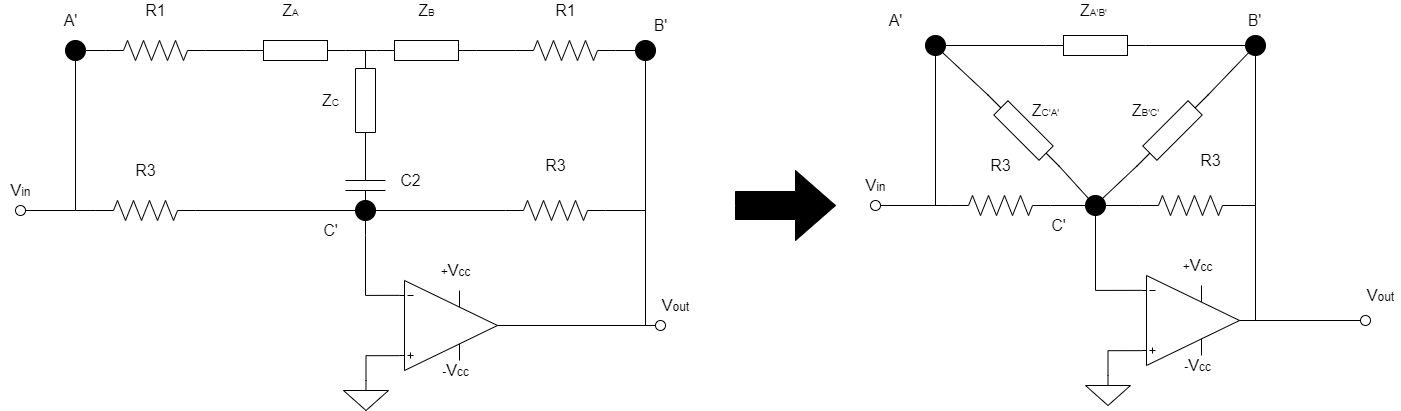
\includegraphics[scale=0.6]{../Ejercicio4-EcualizadorDeFase/Informe/2cambioTriangulo.png}
	\label{2reemplazo} 
\end{figure}


Para no complicar los cálculos se uso el programa Maple para poder obtener los resultados finales de los reemplazos, dejando asi las siguientes impedancias:

\begin{align}

	\begin{equation}
		Z_{1}= 
	\end{equation}

	\begin{equation}
		Z_{2}= R_1 + Z_{B}
	\end{equation}
	
	\begin{equation}
		Z_{3}= \frac{1}{sC_1} + Z_{C}
	\end{equation}

\end{align}




